
\subsection{Segnale e rumore}

Prima di passare alla misura finale analizziamo lo spettro del segnale e lo confrontiamo con quello del rumore per trovare il miglior punto di lavoro.
Per fare questa misura studiamo segnale e rumore del PMT5 servendoci delle funzioni logiche mostrate in \autoref{anti_prov}: per le misure in coincidenza usiamo la funzione (PM6 $+$ PM4) $\&$ PM5 e per quelle in anticoincidenza usiamo 
(PM6 $+$ PM4) $\neg$ PM5.

\marginpar{figura provvisoria}
\begin{figure}[h]
\centering
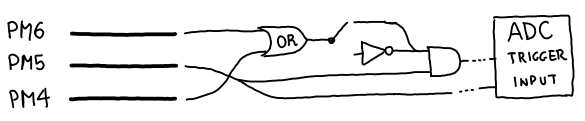
\includegraphics[width=8 cm]{anti_prov}
\caption{schema dei collegamenti utilizzati rispettivamente per le misure in coincidenza ed anticoincidenza.}
\label{anti_prov}
\end{figure}

Abbiamo acquisito i dati in entrambe le configurazioni spaziando da \SI{1600}{V} a \SI{2000}{V} con un intervallo di \SI{50}{V}. In \autoref{quattro} ne mostriamo i principali istogrammi.

\begin{figure}[h]
\hspace{-2cm}
{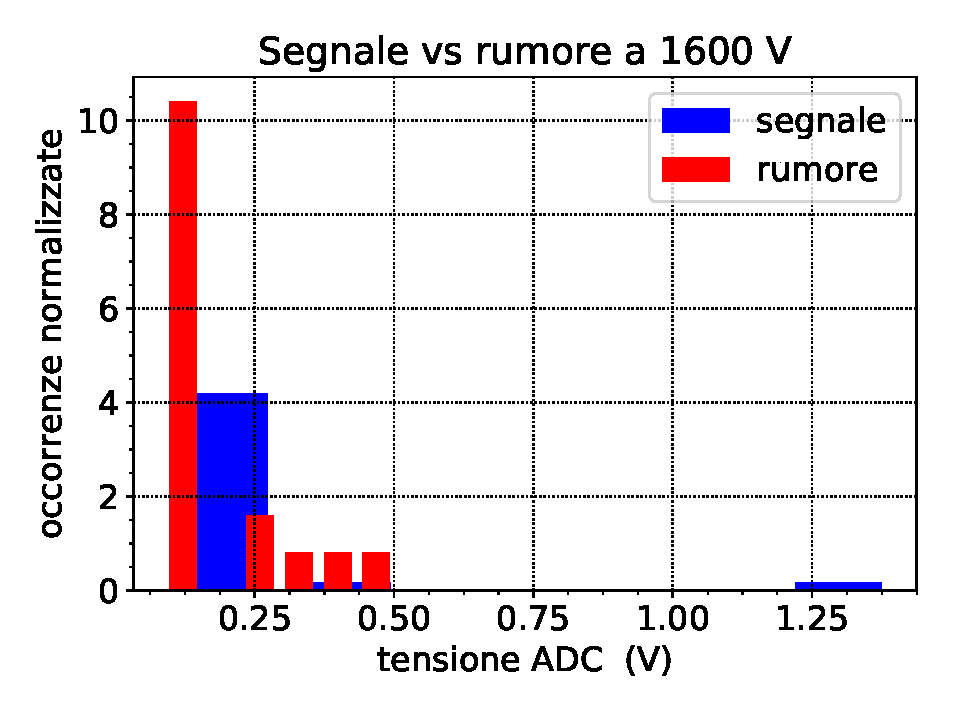
\includegraphics[width=8 cm]{1600}}
\qquad
{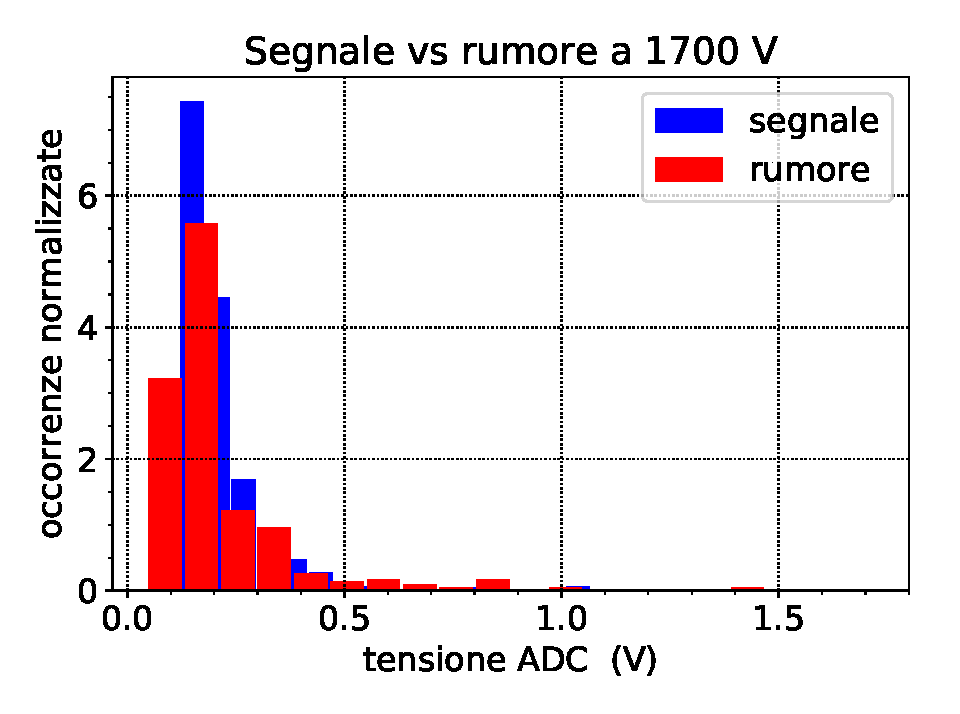
\includegraphics[width=8 cm]{1700}} 

\hspace{-2cm}
{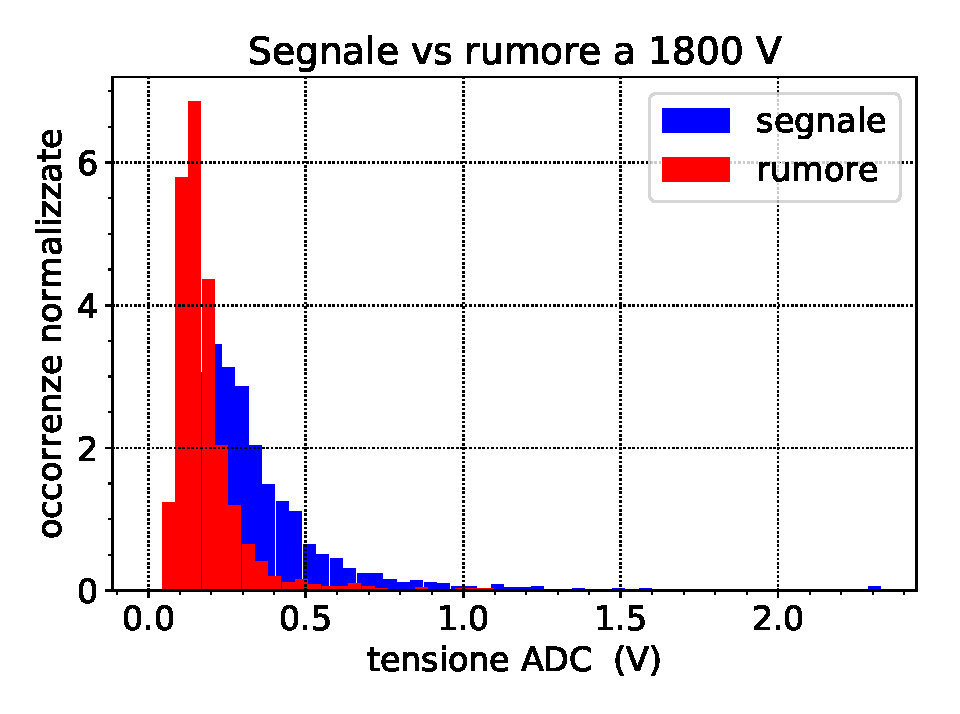
\includegraphics[width=8 cm]{1800}}
\qquad
{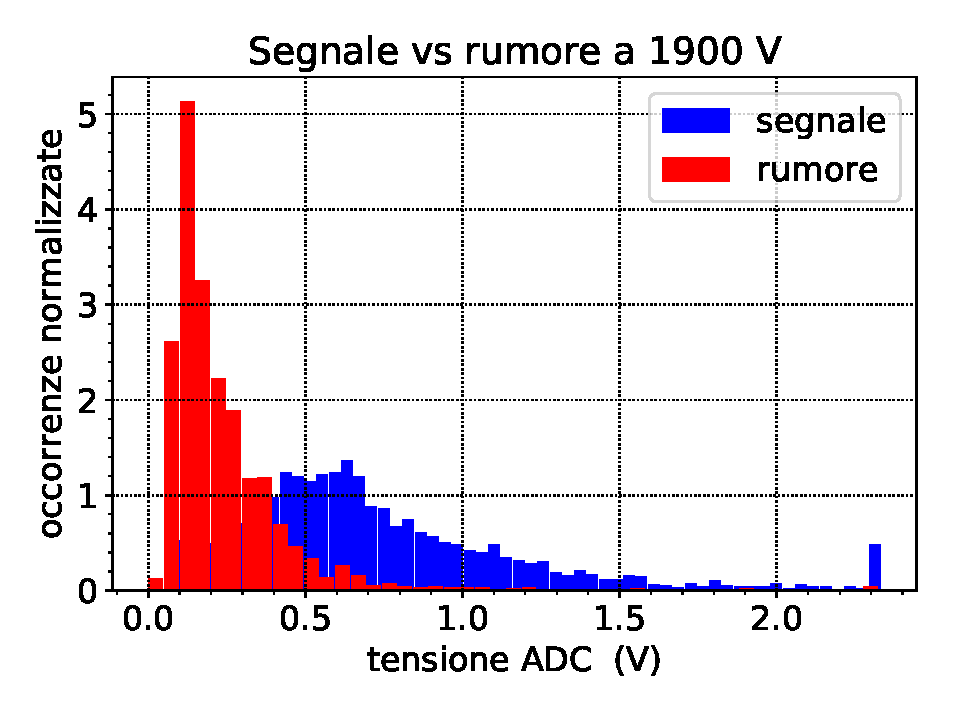
\includegraphics[width=8 cm]{1900}}
\caption{istogrammi che rappresentano il variare degli spettri di segnale e rumore per le tensioni più significative.}
\label{quattro}
\end{figure}

Particolare attenzione merita il confronto tra segnale e rumore per una tensione di alimentazione di \SI{2000}{V} (\autoref{bump}): segnale e rumore sono molto distinti, ma nell'istogramma del segnale si nota un picco nella regione ad elevato rumore.
Esso comprende il $17.7\pm0.7\%$%
\footnote{L'area del picco è stata calcolata eseguendo il rapporto tra il numero di eventi in esso e quelli totali. Questo rapporto è stato eseguito con i conteggi della distribuzione non normalizzata in quanto la somma di variabili poissoniane è ancora una variabile poissoniana. L'errore sul rapporto è dato dalle solite formule di propagazione dell'errore.}
di tutti gli eventi ed è di molto superiore al rate di coincidenze casuali attese che, in tutte le misure, ammontano a meno dell'1\%.
\marginpar{E se facessimo gli istogrammi del rapporto S/N? Premessa: non lo so fare perché quando usi histogram puoi dividere le occorrenze, ma cosa ci fai con l'array ``edges''?}

\begin{figure}[h]
\centering
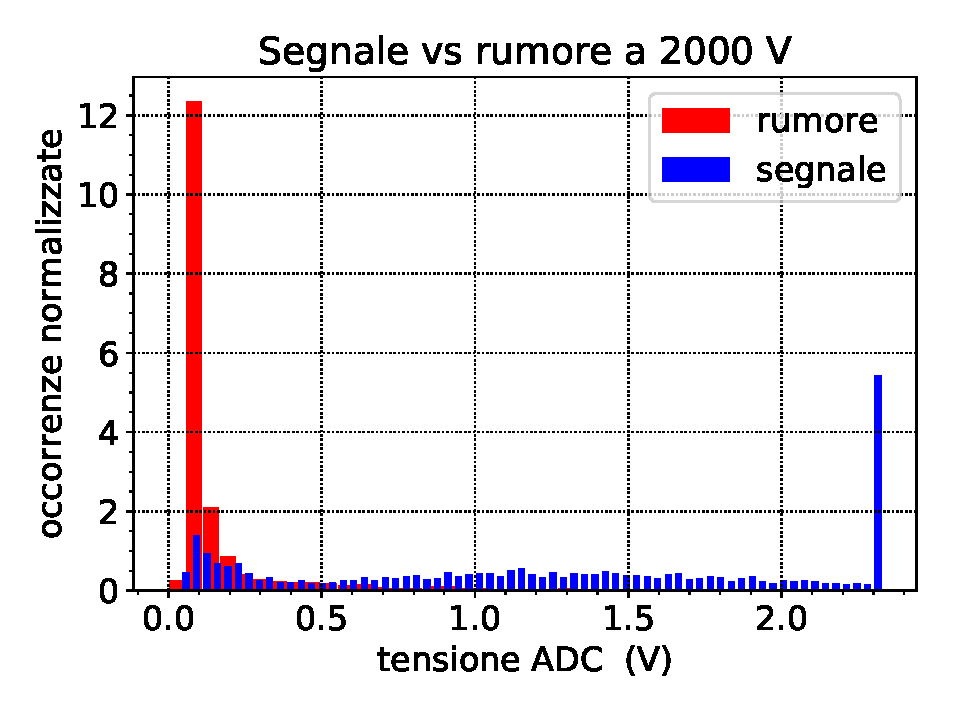
\includegraphics[width=23em]{2000}
\caption{spettro di segnale e rumore a 2000\,V. Sulla sinistra si può notare un picco nella regione ad alto rumore.}
\label{bump}
\end{figure}
